\documentclass[a4paper,12pt]{report}

\usepackage{alltt, fancyvrb, url}
\usepackage{graphicx}
\usepackage[utf8]{inputenc}
\usepackage{float}
\usepackage{hyperref}

% Questo commentalo se vuoi scrivere in inglese.
\usepackage[italian]{babel}

\usepackage[italian]{cleveref}

\title{Relazione del progetto di\\Programmazione ad Oggetti\\``Object One Piece''}

\author{De Tommaso Tommaso\\Giorgini Matteo\\Grimaldi Leonardo\\Scorza Edoardo}
\date{\today}


\begin{document}

\maketitle

\tableofcontents

\chapter{Analisi}	

\section{Requisiti}

Il nostro progetto, richiesto per l'esame di Programmazione ad Oggetti, consiste in un videogioco di battaglie tra navi a tema One Piece.

\subsubsection{Requisiti funzionali}
\begin{itemize}
	\item Il gioco è strutturato a turni, dove le mosse si alternano tra giocatore e nemici.
	\item Il giocatore controlla una nave con cui può navigare all'interno della mappa e interagire con essa
	attaccando i nemici, evitando le mine, raccogliendo i barili per guadagnare esperienza e attraccando alle isole per curarsi e salvare.
	Inoltre, l'esperienza raccolta dai barili potrà essere utilizzata per riparare la nave.
	\item Le navi nemiche hanno il compito di seguire ed attaccare la nave del giocatore.
	\item La mappa di gioco si genera in modo casuale e quindi il gioco prosegue all'infinito.
\end{itemize}

\subsubsection{Requisiti non funzionali}
\begin{itemize}
	\item L'interfaccia grafica deve essere scalabile.
	\item Il turno dei nemici deve essere calcolato in tempi brevi.
\end{itemize}

\section{Analisi e modello del dominio}

Il mondo di gioco è diviso in sezioni che possono essere generate casualmente o caricate, se precedentemente salvate.
%
Ogni sezione contiene il giocatore ed altre eventuali entità che possono essere: nemici, barili, mine ed isole.
%
Il giocatore deve potersi muovere nella sezione corrente e deve poterla cambiare navigando nei bordi.
%
Tutte le navi, che siano nemici o il giocatore, devono collidere con altre navi o entità.
%
Devono inoltre poter sparare e danneggiare le altre navi.
%
Il colpo sparato da una nave deve poter sorvolare i barili e le mine presenti lungo la traiettoria, ma non le altre navi e le isole.
%
Una nave è composta da quattro componenti che sono: la chiglia, la prua, la vela e l'arma.
%
Ognuno contribuisce ad una diversa abilità e la loro distruzione ne comporta quindi la perdità.
%
Le isole, i barili e le mine devono eseguire determinate azioni alla collisione.
%
Le mine dovranno procurare danno alle navi che collidono, i barili invece daranno dell'esperienza al giocatore che vi collide.
%
Le isole, invece, dovranno riparare la nave del giocatore che vi ha colliso e salvare lo stato del gioco.
%
Quando si parla di "salvare", si intende un checkpoint, ovvero l'abilità del giocatore di rinascere dove si è salvato.
%
La possibilità di salvare lo stato del gioco per riprenderlo in un secondo momento dopo la sua chiusura non è prevista.
%
I nemici devono vedere e seguire il giocatore, se questo entra nel loro raggio visivo.
%
I nemici devono anche sparare al giocatore, se questo entra nel raggio dell'arma.
%
I nemici non seguono il giocatore se cambia sezione.

\begin{figure}[H]
	\centering{}
	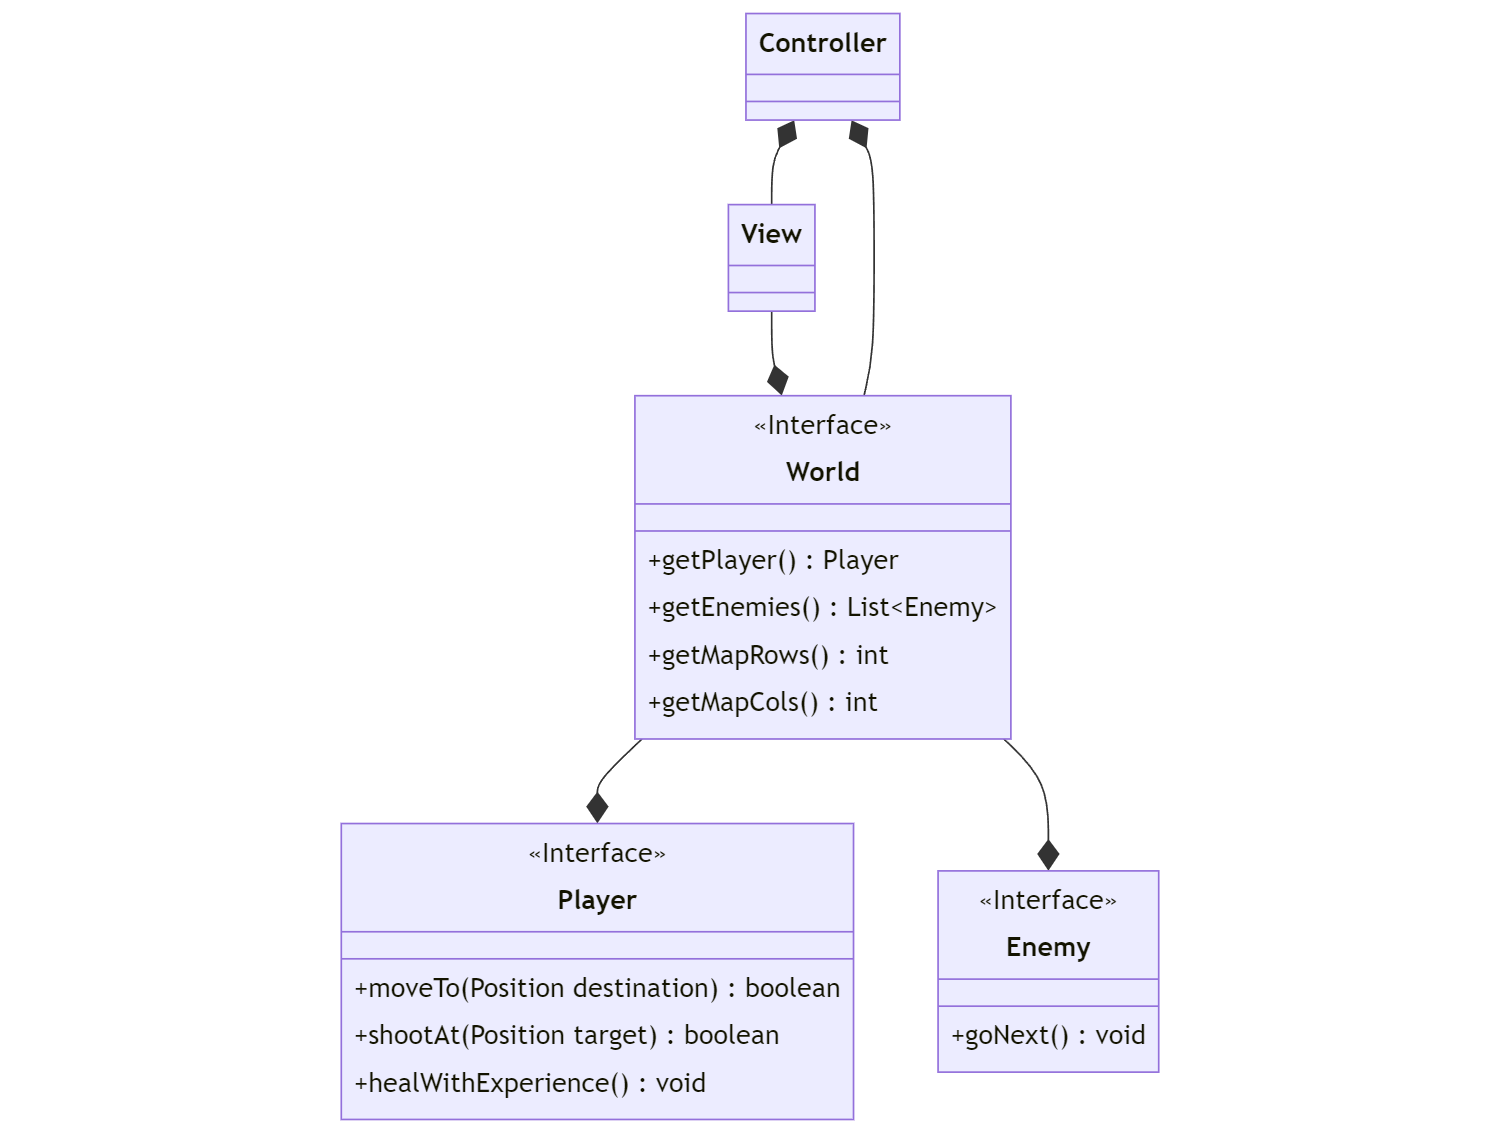
\includegraphics[width=\textwidth]{img/Analysis.png}
	\caption{Schema UML dell'analisi del progetto}
	\label{img:Analysis}
\end{figure}

\chapter{Design}

\section{Architettura}

L'architettura del progetto segue il pattern architetturale MVC.
%
Più nello specifico, la View si occupa di visualizzare a schermo lo stato corrente del gioco,
il Controller si occupa di gestire gli input del giocatore ed agire di conseguenza, ed
il Model si occupa unicamente della logica che definisce il gioco.

Grazie a questa architettura è molto più semplice modificare o cambiare completamente la View
senza conoscere, né modificare, l'architettura interna del Model.
%
Inoltre, il nostro gioco è strutturato per essere a turni ed è quindi "passivo", modificando il suo stato solo dopo un'input,
tuttavia la logica dei turni è stata implementata nel Controller e questo potenzialmente ci permette di usare lo stesso Model
anche per una versione del gioco in tempo reale che sarebbe quindi "attiva", dove il gioco non aspetta l'input dell'utente.

\begin{figure}[H]
	\centering{}
	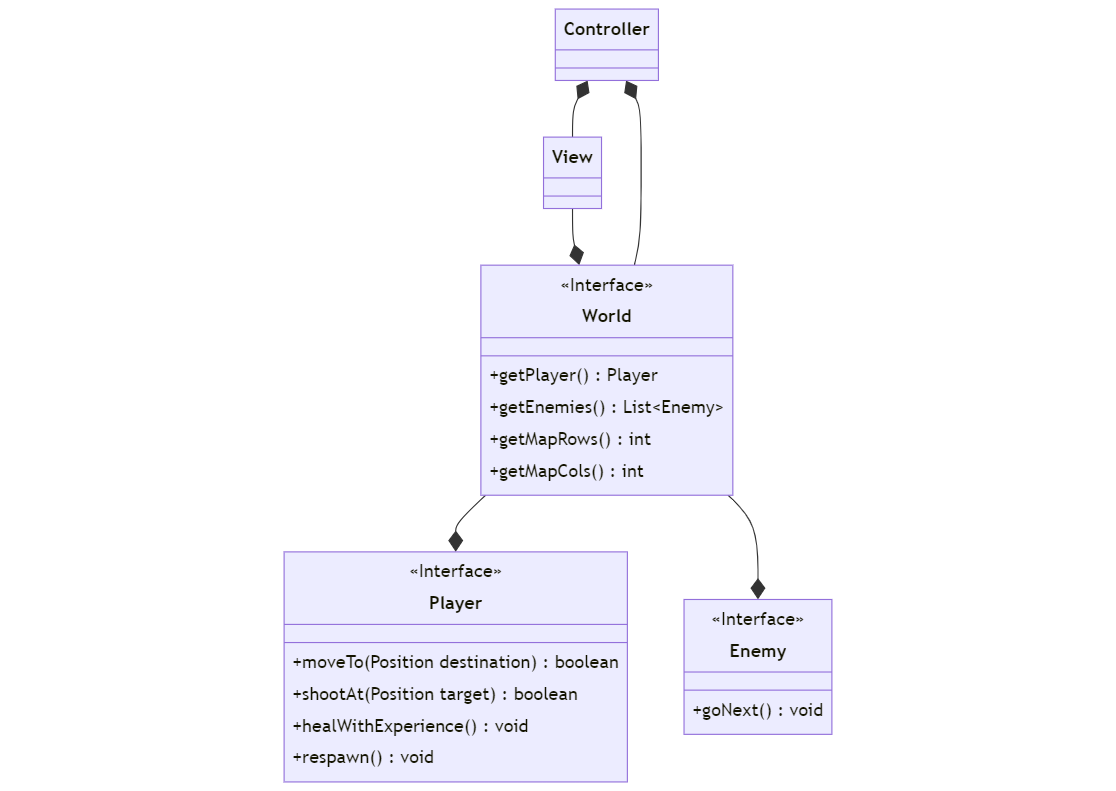
\includegraphics[width=\textwidth]{img/Architecture.png}
	\caption{Schema UML dell'architettura del progetto}
	\label{img:Architecture}
\end{figure}

\section{Design dettagliato}

\subsection*{Tommaso De Tommaso}
\begin{figure}[H]
	\centering{}
	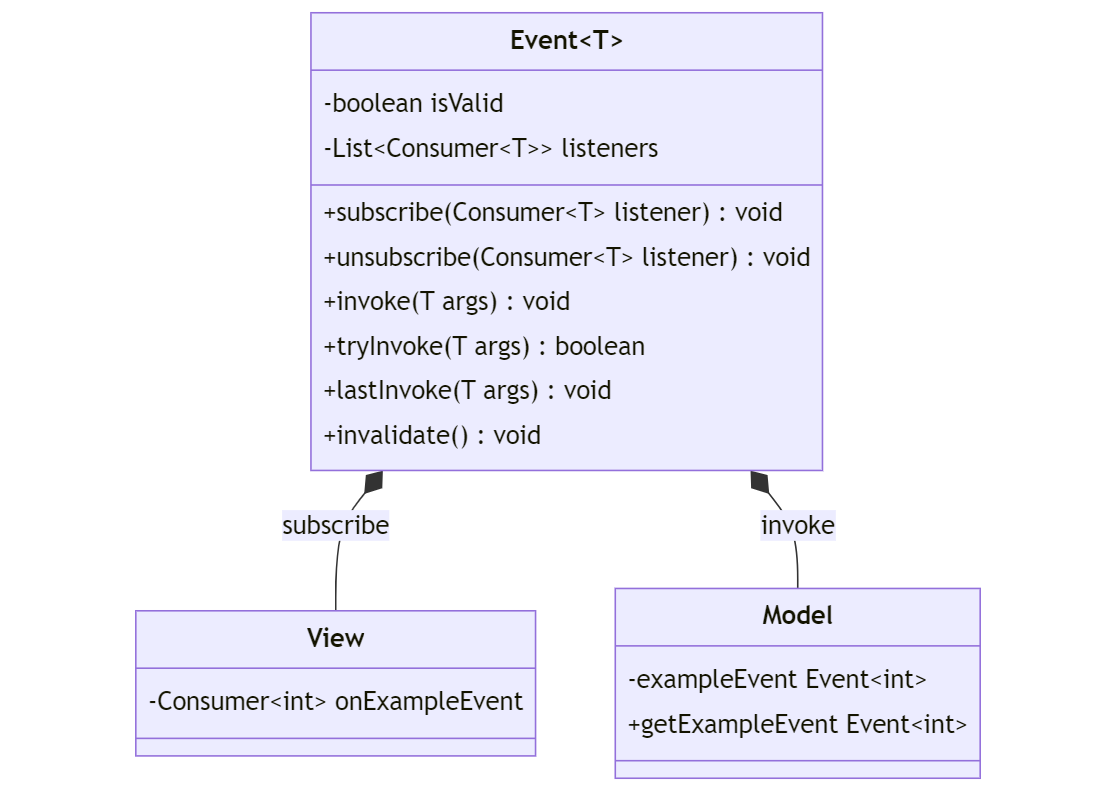
\includegraphics[width=\textwidth]{img/Event.png}
	\caption{Rappresentazione UML della classe Event con una View ed un Model ad-hoc ed un esempio di utilizzo}
	\label{img:Event}
\end{figure}
\subsubsection*{Aggiornamento della View}
\paragraph{Problema} Il Model deve poter comunicare alla View quando e come aggiornarsi senza dover esporre la sua struttura interna.
\paragraph{Soluzione} Usare l'\textit{Observer pattern} per creare un oggetto generico e riutilizzabile che si occupi, nel nostro caso, di informare la View.
%
Questo approccio garantisce anche che View e Model siano "loosely coupled".

\subsubsection*{Salvataggio del gioco}
\begin{figure}[H]
	\centering{}
	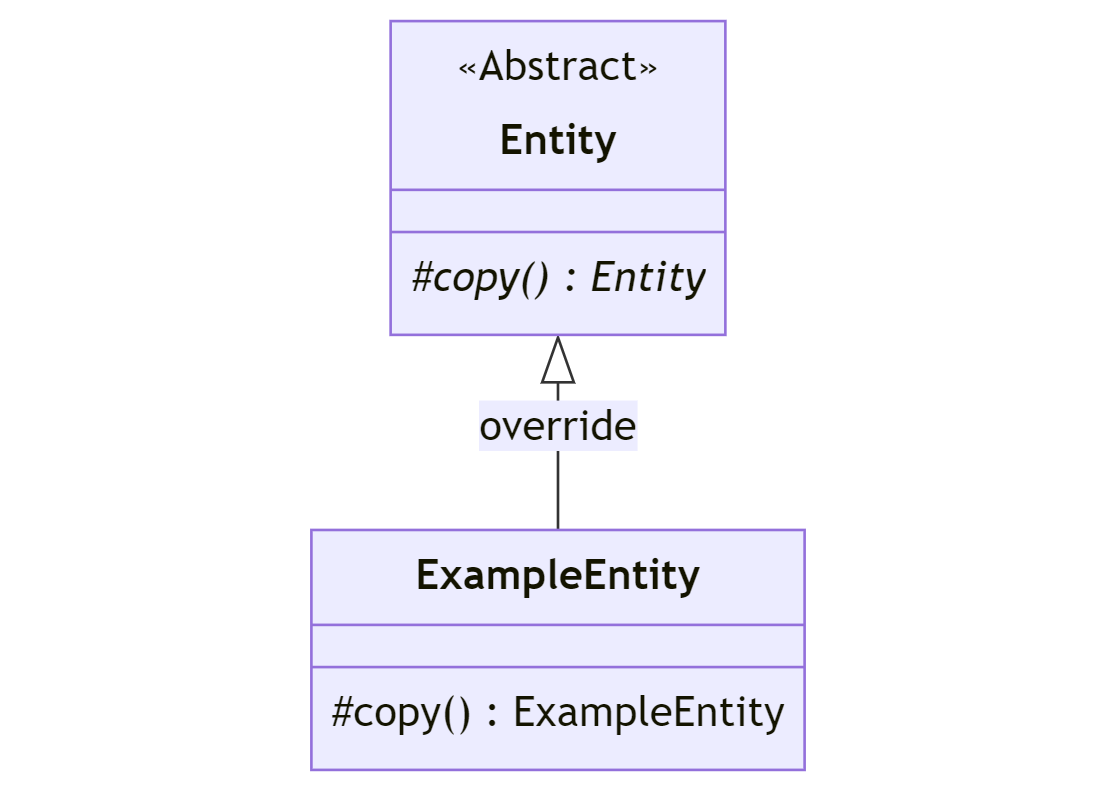
\includegraphics[width=\textwidth]{img/Prototype.png}
	\caption{Rappresentazione UML della classe Entity con un ExampleEntity che eredita da questa e implementa il metodo astratto "copy"}
	\label{img:Prototype}
\end{figure}
\paragraph{Problema} Il Model deve poter salvare il suo stato, questo implica la copia dello stato di ogni entità piuttosto che la copia del suo riferimento.
\paragraph{Soluzione} Usare il \textit{Prototype pattern} per delegare il processo di copia alle entità stesse, con un metodo astratto "copy" nella classe Entity e la sua implementazione in ogni classe che la estende.

\subsection*{Matteo Giorgini}
\subsubsection*{Composizione della nave}

\begin{figure}[H]
	\centering{}
	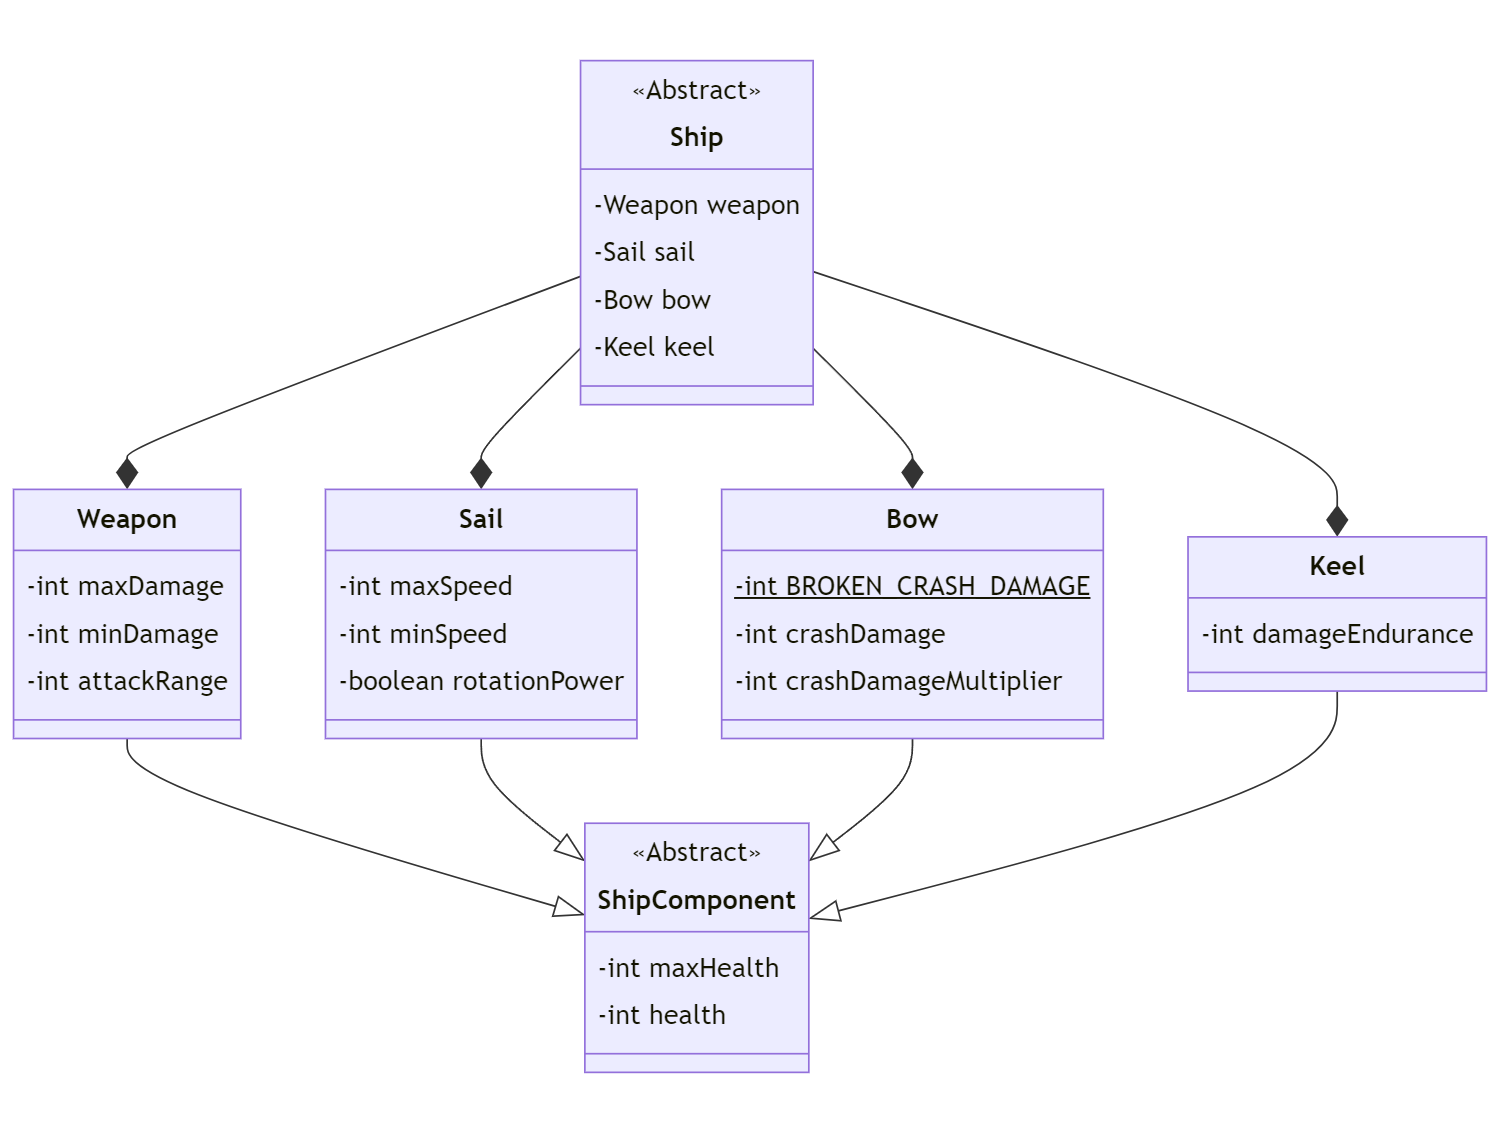
\includegraphics[width=\textwidth]{img/Ship.png}
	\caption{Rappresentazione UML del Composite pattern per la composizione della nave}
	\label{img:Ship}
\end{figure}

\paragraph{Problema} Una nave è composta da varie parti che si occupano di compiti differenti.
\paragraph{Soluzione} Usare il \textit{Composite pattern} per creare un componente composito che contiene i riferimenti ad i vari componenti della nave (Weapon, Sail, Bow, Ship).
%
Ogni componente svolge una funzione differente e alla sua rottura causa un malus alla nave.
%
Questo sistema permette di avere una nave eventualmente estendibile.
\subsubsection*{Costruzione di componenti con statistiche diverse}

\begin{figure}[H]
	\centering{}
	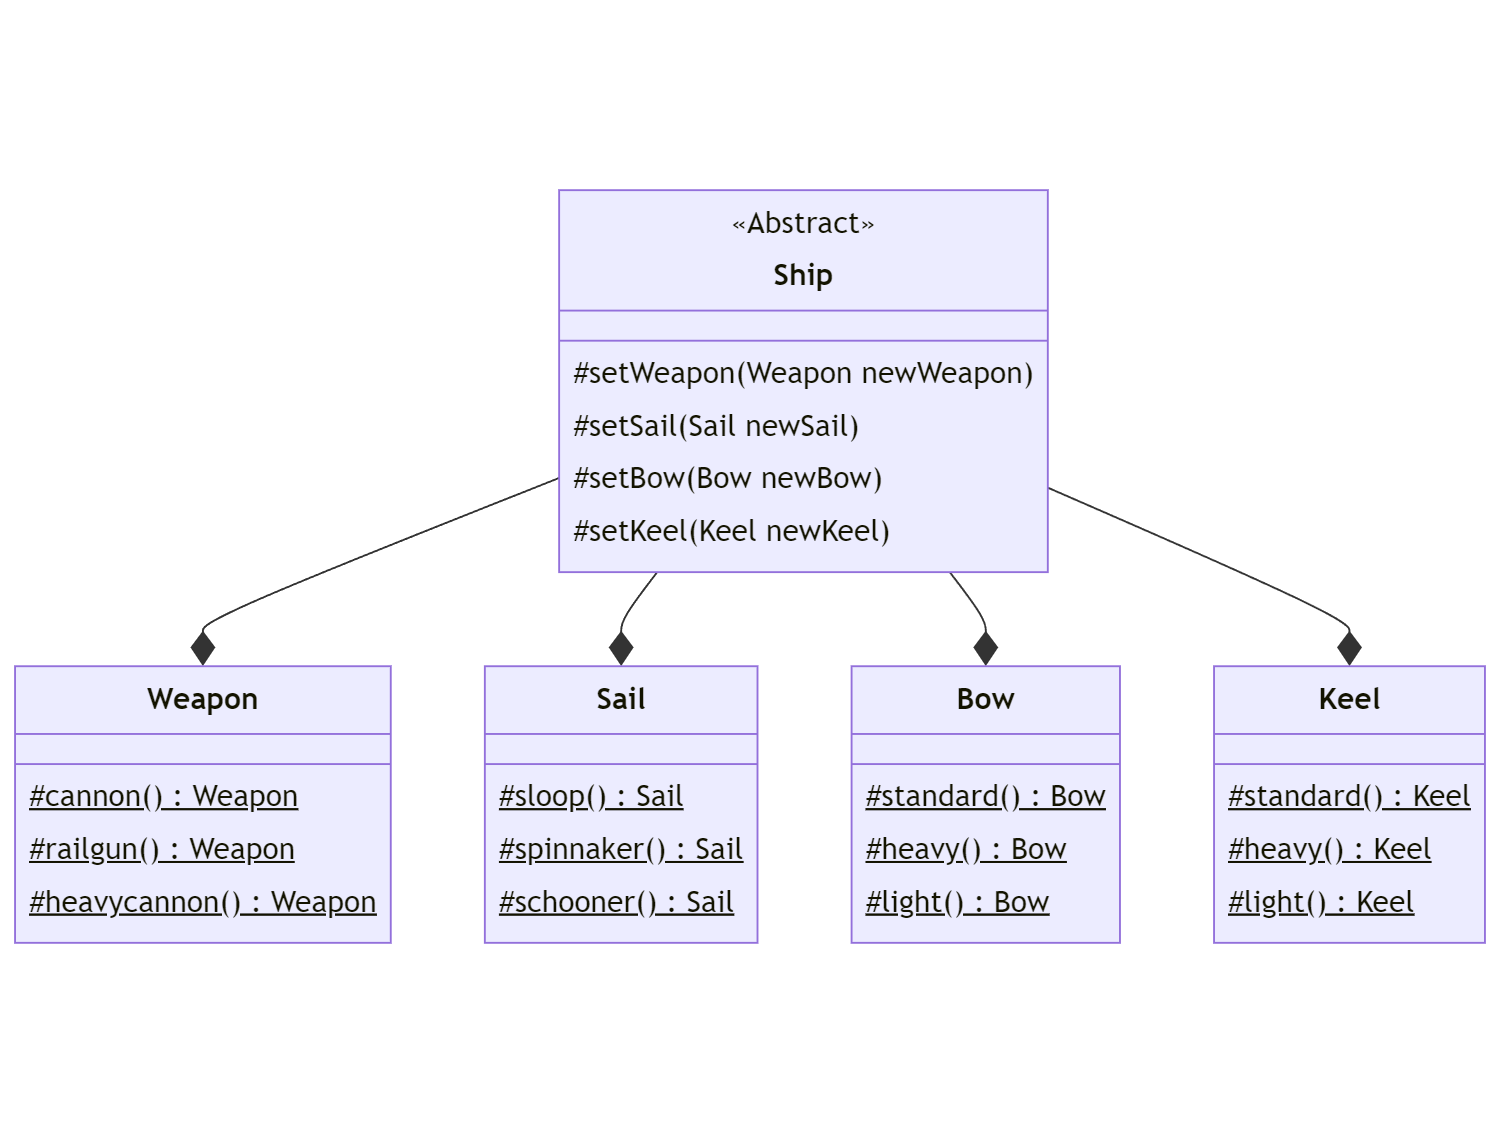
\includegraphics[width=\textwidth]{img/Factory.png}
	\caption{Rappresentazione UML del Factory pattern per la composizione della nave}
	\label{img:Factory}
\end{figure}

\paragraph{Problema} I componenti di una nave possono avere statistiche differenti.
\paragraph{Soluzione} Usare il \textit{Factory pattern} per creare configurazioni diverse di componenti con statistiche diverse.
%
Ogni componente possiede al suo interno dei metodi che costruiscono il suddetto componente con valori differenti e incapsulano il costruttore.

\subsection*{Leonardo Grimaldi}
\subsubsection*{Barra di progresso}
\paragraph{Problema} La view deve rappresentare barre di vita con la stessa struttura, ma colori o proprietà diverse.
\paragraph{Soluzione} Usare il \textit{Decorator pattern} per creare una barra di progresso basilare che può essere assegnata colori diversi, associato un nome, aggiornata con il progresso e che restituisce il componente pronto per essere rappresentato. La classe astratta che fa da Decorator è \texttt{ProgressBarDecorator}, mentre le sue implementazioni sono 

\subsubsection*{Tracciamento del player e dei nemici}
\paragraph{Problema} Consentire al Controller di accedere al \texttt{Player} e alla lista di \texttt{Enemy} senza smascherare la struttura complessa interna del \texttt{World}
\paragraph{Soluzione} Si è deciso di usare il Facade pattern per creare una interfaccia \texttt{World} che contenesse un metodo \texttt{getPlayer()} che ritornasse il \texttt{Player} e un metodo \texttt{getEnemies()} che ritornasse una lista di \texttt{Enemy}. Il Controller in questo modo non dovrà preoccuparsi di come vengono generate le sezioni oppure quale sia quella corrente: riceve subito le entità in quella presente per comodamente gestirne i turni. Alternativamente, avremmo potuto consentire al Controller di accedere direttamente al \texttt{WorldImpl} e le \texttt{Section}, ma avremmo violato principi di incapsulazione permettendo comportamenti indesiderati.

\subsubsection*{Caricamento di una mappa/sezione salvata}
\paragraph{Problema} 
\paragraph{Soluzione}

\subsection*{Edoardo Scorza}
\subsubsection*{AI delle Entità Enemy}
\begin{figure}[H]
	\centering{}
	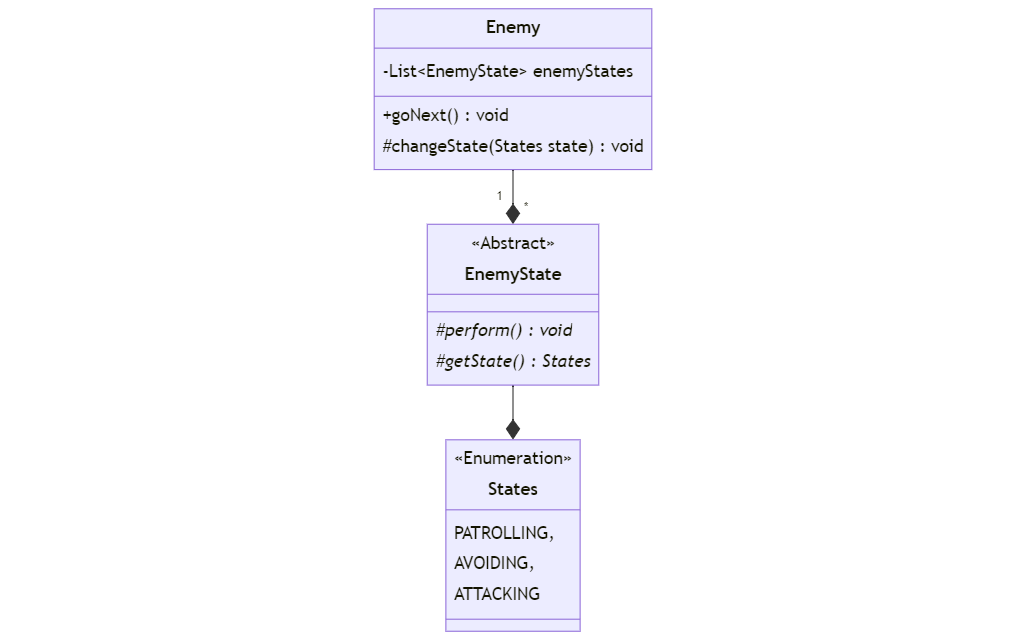
\includegraphics[width=\textwidth]{img/Enemy.png}
	\caption{Rappresentazione UML dello State pattern dell'Enemy}
	\label{img:Enemy}
\end{figure}
\paragraph{Problema} realizzare un sistema di algoritmi in grado di manovrare una Ship, al fine di navigare nella mappa ed attaccare il Giocatore in prossimità di essa.
\paragraph{Soluzione} Ho deciso di optare per uno State pattern, ciò consente di separare le diverse logiche dall'Enemy e dalle logiche stesse, consentendo sia di creare algoritmi volti a una singola situazione ma anche facili da intercambiare.

\subsubsection*{Controller}
\begin{figure}[H]
	\centering{}
	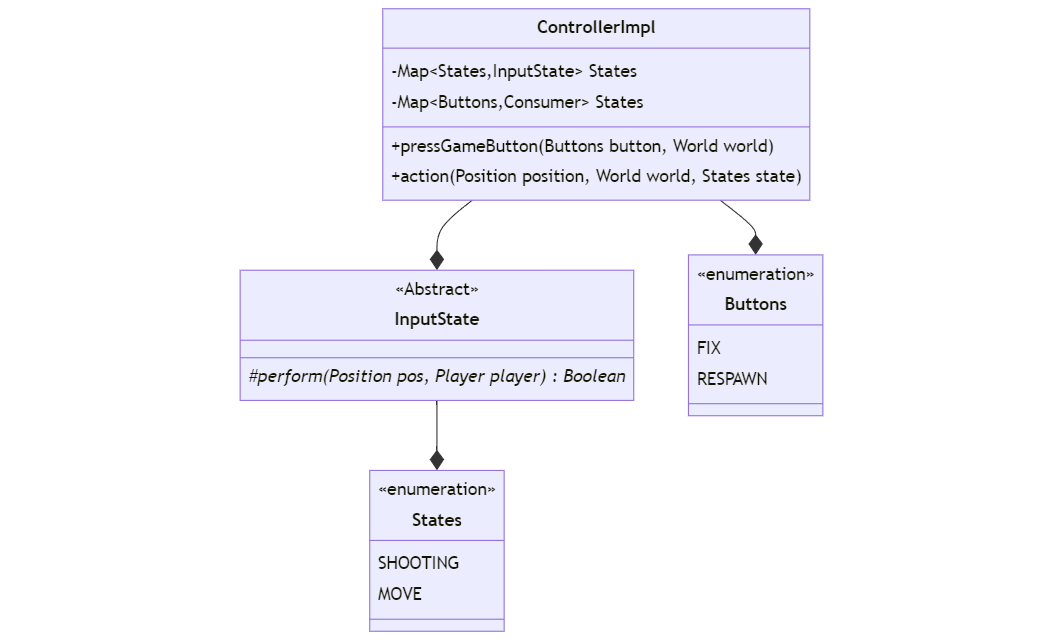
\includegraphics[width=\textwidth]{img/Controller.png}
	\caption{Rappresentazione UML del Strategy pattern usato dal controller per gestire gli input}
	\label{img:Controller}
\end{figure}
\paragraph{Problema} realizzare un controller che oltre a scandire il tempo del model, esponesse in modo chiaro le funzionalità del model in poche, semplici funzioni.
\paragraph{Soluzione} Per l'input di gioco ho utilizzato uno Strategy pattern, atto alla separazione delle due varianti di input richieste dal nostro gioco: muoversi o sparare, in modo simile anche per la gestione di funzionalità del model collegabili a pulsanti esterni, attraverso l'uso di una mappa.

\chapter{Sviluppo}
\section{Testing automatizzato}

Abbiamo eseguito dei testing utilizzando la suite di JUnit.
%
\begin{itemize}
	\item NavigationSystemTest.java testa la capacità del navigation system implementato ( compass ) di dare la direzione corretta per raggiungere un obbiettivo
	\item UtilsTest.java esegue i test di tutti i metodi di Position e Bound in Utils.
\end{itemize}

\section{Note di sviluppo}

\subsection*{Tommaso De Tommaso}
\subsubsection{Utilizzo di una "custom" \texttt{Annotation} }
Permalink: \url{https://github.com/thethunderingmarmot/OOP23-objectonepiece/blob/f1c77c3f045ecd5f6e5b50d53eaae92590d2c32e/src/main/java/it/unibo/object_onepiece/model/PlayerImpl.java#L14}
\subsubsection{Utilizzo di \texttt{Stream}, \texttt{Function} e lambda expressions}
Permalink: \url{https://github.com/thethunderingmarmot/OOP23-objectonepiece/blob/f1c77c3f045ecd5f6e5b50d53eaae92590d2c32e/src/main/java/it/unibo/object_onepiece/model/PlayerImpl.java#L111-L138}

\subsection*{Matteo Giorgini}
\subsubsection{Utilizzo di \texttt{Stream} e lambda expressions}
Usate pervasivamente. Il seguente è un singolo esempio.
Permalink: \url{https://github.com/thethunderingmarmot/OOP23-objectonepiece/blob/b935812786b9f4b2bf504b8380732d7609243f66/src/main/java/it/unibo/object_onepiece/model/Ship.java#L350C1-L353C123}

\subsubsection{Utilizzo di \texttt{BiPredicate} dalla libreria java.util.function}
Permalink: \url{https://github.com/thethunderingmarmot/OOP23-objectonepiece/blob/b935812786b9f4b2bf504b8380732d7609243f66/src/main/java/it/unibo/object_onepiece/model/Ship.java#L391C1-L396C11}

\subsubsection{Utilizzo di \texttt{URL} dalla libreria java.net}
Permalink: \url{https://github.com/thethunderingmarmot/OOP23-objectonepiece/blob/c3fa6ef0fc6adadd4db29c2110c899c068c49ea8/src/main/java/it/unibo/object_onepiece/view/Sound.java#L32C1-L38C7}

\subsubsection{Utilizzo della libreria javax.sound}
Utilizzata in vari punti. Un esempio è il seguente. 
Permalink: \url{https://github.com/thethunderingmarmot/OOP23-objectonepiece/blob/c3fa6ef0fc6adadd4db29c2110c899c068c49ea8/src/main/java/it/unibo/object_onepiece/view/Sound.java#L52C1-L54C45}

\subsubsection{Utilizzo di \texttt{Logger} dalla libreria java.util.logging}
Permalink: \url{https://github.com/thethunderingmarmot/OOP23-objectonepiece/blob/c3fa6ef0fc6adadd4db29c2110c899c068c49ea8/src/main/java/it/unibo/object_onepiece/view/Sound.java#L56C1-L56C56}

\subsection*{Leonardo Grimaldi}

\subsubsection{Utilizzo dell'algoritmo di \textit{White noise} dalla libreria JNoise}

Permalink: \url{https://github.com/thethunderingmarmot/OOP23-objectonepiece/blob/7a0137595ea7d9762cb942ab84609625c92ad2cc/src/main/java/it/unibo/object_onepiece/model/Section.java#L85C9-L86C22}

\subsubsection{Utilizzo di \texttt{GridView} e \texttt{GridModel} dalla libreria Grid}

Permalink: \url{https://github.com/thethunderingmarmot/OOP23-objectonepiece/blob/6e21ea8b2bcbecf144d98e7dac5f3d1b23f450d8/src/main/java/it/unibo/object_onepiece/view/ObjectOnePiece.java#L156C5-L176C6}

\subsubsection{Utilizzo della libreria JavaFX}

Permalink: \url{https://github.com/thethunderingmarmot/OOP23-objectonepiece/blob/6e21ea8b2bcbecf144d98e7dac5f3d1b23f450d8/src/main/java/it/unibo/object_onepiece/view/ProgressBarImpl.java#L27C5-L59C6}

\subsubsection{Utilizzo di \texttt{BiFunction} dentro una \texttt{Map}}

Permalink: \url{https://github.com/thethunderingmarmot/OOP23-objectonepiece/blob/6ae9d20e3d3e9858b3098309406cf93128f788fd/src/main/java/it/unibo/object_onepiece/model/Section.java#L35C5-L41C8}

\subsubsection{Utilizzo di \texttt{Stream}, \texttt{Optional} e lambda expressions}

Permalink: \url{https://github.com/thethunderingmarmot/OOP23-objectonepiece/blob/6ae9d20e3d3e9858b3098309406cf93128f788fd/src/main/java/it/unibo/object_onepiece/model/Section.java#L131C1-L142C6}

\subsection*{Edoardo Scorza}
\subsubsection{Lambda e supplier per la costruzione di una Mappa}
Permalink: \url{https://github.com/thethunderingmarmot/OOP23-objectonepiece/blob/c3fa6ef0fc6adadd4db29c2110c899c068c49ea8/src/main/java/it/unibo/object_onepiece/model/Compass.java#L16C1-L26C7}

\subsubsection{Consumer}
Permalink: \url{https://github.com/thethunderingmarmot/OOP23-objectonepiece/blob/805803a2ce3b2c9844d0cecb63fac15f8a5d2780/src/main/java/it/unibo/object_onepiece/controller/ControllerImpl.java#L20C4-L22C7}

\subsubsection{Stream}
Permalink: \url{https://github.com/thethunderingmarmot/OOP23-objectonepiece/blob/805803a2ce3b2c9844d0cecb63fac15f8a5d2780/src/main/java/it/unibo/object_onepiece/controller/ControllerImpl.java#L26C9-L28C10}	


\chapter{Commenti finali}

\section{Autovalutazione e lavori futuri}

\subsection*{Tommaso De Tommaso}
Questo progetto è stata un'ottima occasione più per "sviluppare" me stesso che il gioco in sé.
%
La mia parte consisteva nello sviluppo del Player, del Barrel e dell'Island.
%
Inoltre, dovevo sviluppare anche il sistema di salvataggio del gioco, siccome collegato alle Island.
%
Tutto ciò è stato terminato prima del previsto ed ho quindi pensato di aver sovrastimato la mia parte.
%
Temendo di non raggiungere la quota di 70 ore, ho proseguito nell'aggiunta di feature opzionali, rimanendo nei limiti del progetto, invece di fare testing.
%
Fino a quel momento, infatti, nessun test era stato fatto a causa dell'erroneo sentimento maggioritario, nonché il mio, di testare il gioco giocandolo, non appena la View fosse stata completata.
%
Inevitabilmente, quando ciò è accaduto, ci siamo ritrovati sommersi da bug e comportamenti inaspettati.
%
Questo ha provocato diversi aggiustamenti "dell'ultimo minuto" che non hanno ricevuto la cura del resto del progetto.
%
Oltre a questo, nella foga di aggiungere feature opzionali, si è deragliati molto dalla progettazione iniziale, causando diverse discordie.
%
Queste cose, da perfezionista quale sono, mi hanno dato non poco fastidio, ma, dopotutto, la colpa è per lo più mia.
%
Non penso di portare avanti questo progetto poiché, citando la meta-relazione, a mio avviso non è affatto "sufficientemente ben riuscito da poter esser usato come dimostrazione di esser capaci progettisti", ma anzi è un esempio da non imitare.

\subsection*{Matteo Giorgini}
La realizzazione di questo progetto è stata un grande insegnamento sul lavoro di gruppo.
%
Sono soddisfatto della parte che ho svolto nonostante ci siano stati molti cambiamenti in corso d'opera, probabilmente a causa di una progettazione non troppo dettagliata.
%
Il mio ruolo consisteva nella realizzazione dell'entità come elemento generale e della nave (movimento, combattimento, collisioni, etc.).
%
Inizialmente ho sottostimato i tempi per la realizzazione della mia parte, ed ho quindi implementato successivamente nuove funzionalità come le mine ed i suoni.
%
Successivamente però si sono rivelate più complicate del previsto sempre a causa della progettazione e degli scarsi test e hanno necessitato di vari adattamenti,
che non hanno permesso la totale implementazione di alcune funzionalità opzionali.
%
Nonostante questo la mia parte è risultata flessibile ed estendibile, soprattutto la nave ed i suoi componenti sono modificabili e sono contento di come ho realizzato le meccaniche di movimento, sparo e collisione della nave.
%
Concludo dicendo che questo progetto è stato molto formativo su vari aspetti come confrontarsi per risolvere problemi comuni e risolvere errori in compilazione e eccezioni durante l'esecuzione.
%
In futuro vorrei ultimare l'implementazione dei suoni e rendere possibile ottenere in gioco i componenti con statistiche differenti che ho creato per la nave.

\subsection*{Leonardo Grimaldi}

\subsection*{Edoardo Scorza}

Il mio ruolo nel progetto consisteva nella realizzazione del controller(MVC) e dei nemici,
In generale ho seguito il progetto nella fase di analisi e strutturazione, essendo parte attiva del progetto, ritengo di dover conoscerlo interamente
per contribuire nel modo migliore possibile e, anche perchè la mia parte si basava su quella struttura.
Il problema principale che abbiamo riscontrato è stata la coordinazione di gruppo, essendo il modello MVC, senza una variante di tutti i componenti non eravamo 
in grado di eseguire prove a mano, ne ci siamo preoccupati troppo di eseguire testing automatizzato, ciò ha seguitato a una serie
di riscritture e adattamenti, sicuramente una cosa su cui riflettere.
Fortunatamente ciò non ha precluso il lavoro finale, mi ritengo fortunato, abbiamo sempre discusso assieme a fronte di 
problemi e formulato strategie assieme. Sono abbastanza soddisfatto del mio lavoro, l'uso di pattern e il pensiero alla semplicità, mi hanno permesso
di realizzare un enemy semplice modulabile ed efficace, in minima parte anche il controller, che soprattutto beneficiava delle scelte del model.
Se dovessi pensare a un futuro per questo gioco direi che ci sono tante possibilità, non solo è strutturato come un sandbox, ovvero che estendendo 
le classi astratte è possibile aggiungere nuove entità, ma anche la natura stessa del gioco si può cambiare, potrebbe facilmente diventare Real-Time ( invece che a turni )

\section{Difficoltà incontrate e commenti per i docenti}
\subsection*{Tommaso De Tommaso}
Grazie a questo corso ho potuto scoprire Java che, nonostante conoscessi già abbastanza bene il C\#, desideravo studiare in quanto molto usato in diversi settori.
%
La cosa che mi ha colpito di più di questo corso è il fatto che c'è sempre stato un focus anche sulla programmazione funzionale, su cui ero totalmente ignorante.
%
Questo mi ha permesso di imparare qualcosa di nuovo, nonostante conoscessi già la programmazione ad oggetti.
%
Il mio unico problema è stato adattarmi alla presenza del Type Erasure che ha persino cambiato considerevolmente parte della progettazione di questo progetto.


\appendix
\chapter{Guida utente}

Avviando il gioco, l'utente si troverà sullo schermo una finestra con in centro una griglia azzurra (mappa di gioco) e un HUD (denotato dal testo "Player info") sulla parte destra.
%
Nella griglia di gioco il player è identificato dalla nave più chiara con il teschio sulla vela.
%
Esso si può muovere nelle quattro direzioni premendo con il click sinistro del mouse sulla casella adiacente.
%
Se la nave non è direzionata verso la casella in cui ci si vuole recare, la nave impiegerà un turno per girarsi.
%
Quando il giocatore cerca di muoversi sulle caselle del bordo, si sposta su una sezione diversa del mondo e non potrà più tornare alla precedente ammenoché non l'abbia salvata e sia in seguito ``morto''.
%
Per sparare ad una nave nemica il giocatore deve premere con il click destro nelle celle in linea con i fianchi della nave.
%
Il range di sparo è di 3 caselle sia per il player che per i nemici e il cannone fa un danno AoE (Area of Effect) di 3x3 caselle con il danno maggiore nel centro.
%
È possibile anche speronare una nave nemica mentre si è accanto ad essa cliccandoci sopra con il tasto sinistro del mouse.
%
Se il Keel di una nave è danneggiato, speronandola riceve un maggior danno rispetto a quello di default.
%
Il giocatore può curarsi e salvare su una isola premendo il tasto sinistro mentre è a fianco ad essa.
%
Se il giocatore viene affondato (Keel della nave a zero) per continuare il gioco dovrà premere su una casella e a quel punto respawnerà dove ha salvato oppure in una nuova mappa.
%
\newline
Nel HUD vengono mostrate quattro barre di vita che riguardano la nave:
\begin{itemize}
	\item Weapon: vita dell'arma; raggiunto lo zero il giocatore non potrà più sparare.
	\item Bow: vita della prua; raggiunto lo zero non potrà più speronare.
	\item Sail: vita della vela; raggiunto lo zero non potrà muoversi.
	\item Keel: vita della chiglia; raggiunto lo zero il gioco si fermerà e l'utente dovrà cliccare su una casella per respawnare.
\end{itemize}
Inoltre, sotto alle barre di vita sono presenti tre pulsanti.
%
Il primo con l'icona di una tavola di legno consente al giocatore di riparare la nave (curarsi) utilizzando l'esperienza raccolta dai barili nella mappa.
%
Sotto ad esso si trova un numero che indica quanta esperienza l'utente ha a disposizione per ripararsi. Il costo di cura è 100.
%
Il secondo con la scritta "Respawn" consente al player di rigenerare una nuova mappa oppure tornare all'isola salvata.
%
Il terzo bottone spegne/riaccende gli effetti sonori del gioco.

\chapter{Esercitazioni di laboratorio}
\subsection{leonardo.grimaldi2@studio.unibo.it}

\begin{itemize}
 \item Laboratorio 08: \url{https://virtuale.unibo.it/mod/forum/discuss.php?d=148025#p209751}
\end{itemize}

\bibliographystyle{alpha}
\bibliography{13-template}

\end{document}